\def\year{2018}\relax
%File: formatting-instruction.tex
\documentclass[letterpaper]{article} %DO NOT CHANGE THIS
\usepackage{aaai18}  %Required
\usepackage{times}  %Required
\usepackage{helvet}  %Required
\usepackage{courier}  %Required
\usepackage{url}  %Required
\usepackage{graphicx}  %Required
\frenchspacing  %Required
\setlength{\pdfpagewidth}{8.5in}  %Required
\setlength{\pdfpageheight}{11in}  %Required
%PDF Info Is Required:
  \pdfinfo{
/Title (Not Can We, But Should We: A Design Framework on Appropriate Levels of Automation)
/Author (Chenhao Tan, Brian Lubars)}
\setcounter{secnumdepth}{0}  
 \begin{document}
% The file aaai.sty is the style file for AAAI Press 
% proceedings, working notes, and technical reports.
%
\title{Not Can We, But Should We: \\A Design Framework on Appropriate Levels of Automation}

\author{Chenhao Tan \and Brian Lubars\\
Department of Computer Science\\
University of Colorado, Boulder\\
{chenhao.tan, brian.lubars}@colorado.edu\\
}

%\newcommand{\citet}[1]
%{\citeauthor{#1} ̃\shortcite{#1}}
%\newcommand{\citep}{\cite}
%\newcommand{\citealp}[1]
%{\citeauthor{#1} ̃\citeyear{#1}}

\maketitle
\begin{abstract}
Humans and machines offer complementary abilities. Some tasks are suitable for automation (machine control), some should arguably not be automated (human control), and some are amenable to a mix of the two (human-in-the-loop or machine-in-the-loop designs). What factors go into this classification? When is one paradigm more appropriate than another? By examining factors behind task delegation, human ability, and machine ability for a variety of tasks, we aim to develop a taxonomy of task spaces which help contextualize research and design choices for designing more human-centered automated systems.
\end{abstract}

\section{AI Agents}
Autonomous computer systems that accomplish tasks in dynamic and uncertain environments are increasingly considered with an agent-based design. Key characteristics of an agent-based design include that the system is an entity designed for a specific purpose (achieve a goal), is autonomous, and capable of problem-solving in response to the environment \cite{jennings-2000}. Advantages of such a design are a more unified and powerful interface that abstracts away unnecessary details, and the potential for intelligent cooperation and connection between different systems \cite{bradshaw}

Note: Perhaps we're less concerned with an "agent" design, and more concerned with general autonomous systems? 

Since all alternatives to AI agents are currently human agents, the natural framing of the delegation question is as a choice between the two. Which tasks should AI agents take over, and which are best left to human control? Here we consider both the rational/cognitive factors: a cost-benefit analysis between utility and risk; and the affective factors: 

We are additionally concerned with factors which have implications in the design of automated systems (e.g. interpretability, explanations, trust).

\section{Task Delegation}

\cite{milewski1} proposes a "delegation stance", a term encompassing the complex factor interactions that result in possible delegation to either a human or computer. They find this useful in combining information across disciplines, since much delegation research is between humans. Broadly, delegation factors can be broken down into three categories: delegator characteristics, delegator perception of delegate characteristics, and situational variables.

Prior research indicates that people are willing to delegate in the following scenarios \cite{milewski1}: 
\begin{enumerate}
    \item When the agent is perceived as competent
    \item When the agent is perceived as trustworthy and confident
    \item When the agent is perceived as similar to the delegator
    \item When the delegator is experienced or confident in the situation
    \item When the workload or nature of work necessitates it
    \item When delegation benefits the participants: maximize overall performance and incentive structures, motivation or morale or skill-building in delegate, or building a relationship between the the delegator and the delegate (if human).
\end{enumerate}

Though we are focused on whether a subject is willing to delegate or not, it is worth noting that we are ignoring many situational variables relating to practical delegation. These include the frequency of delegation, the amount of monitoring done by the person delegating \cite{milewski1}, and the workload of delegator \cite{leana1986predictors}.

\section{Task and Human Factors of Delegation}
To explain the human and task factors behind a task delegation decision, we consider a model with four main dimensions: a person's \textbf{motivation} in undertaking the task, their perception of the task's \textbf{difficulty}, their perception of \textbf{risk} associated with accomplishing the task, and finally their \textbf{trust} in the AI agent to accomplish the task. 

% We will explain and motivate each task in more detail later, but first we will explain the high-level interaction between the variables.

%We propose that an AI delegation decision depends on factors related to task traits, task-specific personality traits, and general personality traits.

\subsection{Motivation}
The motivation dimension examines the reasons someone may be interested in accomplishing a given task and to the expected utility that accompanies the task's successful completion. How important is accomplishing this task, and why? Is the task personally meaningful? Is it a stepping-stone to a larger goal, or an end in itself? We further decompose purpose into three sub-factors: the \textbf{intrinsic motivation} or interest, \textbf{goal}, and the \textbf{utility}/importance of the task.

According to Locke, motivation and cognition are collectively responsible for determining action. Motivation is an energizing function that helps initiate and sustain task-related actions, and arises through interactions between a person and the environment \cite{latham2005work}. Motivation can affect action by directing our attention towards achieving values or goals, and by regulating the intensity and persistence of actions. Cognition matters because we can choose which values or goals to act on and adjust our values through thought \cite{Locke-motivation-2000}. Since motivation drives action, people are unlikely to choose self-delegate a task for which they have no motivation if given a choice. This suggests \textbf{intrinsic motivation} to be a likely factor in task delegation.

\cite{thomas-intrinsic-motiv} suggests four cognitions which are responsible for additively producing intrinsic task motivation: impact, competence, meaningfulness, and choice. Competence is similar to Bandura's concept of self-efficacy. We will refer generally to intrinsic task motivation as a factor in delegability, but it is worth keeping in mind the possible variables behind it. Meaningfulness is likely particularly salient when considering task delegation [cite? meaning came up a lot in the class survey]. Practically, Maslow's (1943) hierarchy need theory has modern acceptance in explaining need-based actions, and values are used to explain individual differences in actions in given situations \cite{latham2005work}.

Goal Setting Theory examines the factors behind an effective goal, especially the effects of conscious motivation on performance. Locke et. al. define a goal as "the object or aim of an action." Such effects are strongest when people are more committed to their goals, and goal commitment is suggested to arise from (1) believing the goal outcome is important and (2) higher self-efficacy, discussed later. A belief in goal importance may come from a public commitment, incentives, or motives \cite{locke-goal}. [Accountability may also be considered here]

Generally, a goal may be performance-oriented or mastery-oriented [cite?]. Performance goals emphasize achieving certain external metrics or recognition, while someone with a mastery goal is instead more interested in learning and acquiring skills and strategies. [clarify the distinction btw extrinsically-motivated goals and intrinsic vs this]

[add section on utility or goal importance] 

A decision on the delegation of a given task can vary between individuals. A large part of this variability may be explained by differences in the motivation, values, goals, and utility[cite?]. These factors combined can be summarized as: is the person motivated to actually undertake the task themselves, and does delegating it undermine or support the goal?

\subsection{Difficulty}
We suggest that perceived task difficulty is the second major dimension. Difficulty can be decomposed into three main variables: estimated effort required, estimated abilities required, and self-efficacy.

In a study of insurance claims adjusters, \cite{leana1986predictors} found that subordinates considered to be more "capable, responsible, and trustworthy" were given more authority. Decision importance was also a significant predictor, negatively correlated with authority given.

%Leana, 1986; Keller, 1997).

Self-efficacy comes from Social Cognitive Theory in psychology, which is concerned with the workings of human agency -- how people can bring about changes in their lives \cite{Bandura-agency}. Among the requirements for human agency are self-reactiveness (motivating and constructing courses of action) and self-reflectiveness (personal examination of abilities and pursuits). %Properties of human agency are identified as intentionality, forethought, self-reactiveness, and self-reflectiveness. Self-reactiveness involves motivating and constructing courses of action. The last involves personal examination of abilities and pursuits. 

\cite{Bandura-89} defines self-efficacy as a person's "beliefs about their capabilities to exercise control over events that affect their lives." It can be thought of as a task-specific self-confidence: a high degree of self-efficacy means that an individual is confident in their ability to accomplish a task through effort. Self-efficacy  is partly a reflection of their actual capabilities (performance accomplishments), but it also arises through social persuasion and vicarious experience, and it depends on emotional states \cite{Bandura-89}.

Experience and confidence have been linked with delegation in several studies. This is thought to be because delegation involves a loss of control and an increase of ambiguity \cite{milewski1}, and confidence and experience helps to mitigate those concerns. Situational confidence is similar to self-efficacy.

A perception of difficulty may be poorly calibrated if the person has little experience with the task. If the person does have experience, we propose that self-efficacy is largely correlated with a perception of the task's difficulty. Note that if outcomes are more random or not perceived to be related to effort, then self-efficacy may not be as strongly linked with motivation and action \cite{Bandura-agency}.

Self-efficacy is also thought to affect motivation.  Individuals with low self-efficacy tend to avoid more challenging tasks, while higher self-efficacy can lead to more motivation and higher goals \cite{Bandura-89}.

We propose that self-efficacy can be at least partially explained in terms of personal experience/familiarity with the task and the skills or abilities required. More experience with the task would logically give rise to a deeper understanding of the challenges, strategies, and skills required to complete the task. If the person feels that they have the necessary abilities, then their self-efficacy would rise. [cite]

\subsection{Risk}
Risk is the third major dimension. Risk can be considered as the [cite: definition?]. We propose it is composed of personal \textbf{accountability} for the task outcome, the \textbf{probability of errors}, and the \textbf{cost (or magnitude) of those errors}.

One way to think about delegation is in terms of a rational cost-benefit analysis in which a person attempts to minimize costs and maximize utility when considering the costs, risks, and benefits of each agent \cite{castelfranchi-deleg-1998}. However, if the costs and benifits are uncertain, risk becomes important. In practical evalutations in decisions to delegate between agents, to delegate is to take a risk. It amounts to a bet based on the probability to win or lose and the costs and benefits of the outcomes \cite{castelfranchi-deleg-1998}. 

Lewandowsky et al. (2000) found that trust was a bigger factor in a decision to delegate to automation than to delegate to a person, and suggested that ultimate responsiblity for the delegation may play a role. If people perceive delegation as spreading responsibility, as perhaps they do when delegating to a person, then they may be more likely to delegate. Interestingly, Stout et. al (2014) found users more likely to delegate to an autonomous booking agent as accountability increased, and speculated that perhaps subjects saw the delegation as a means of reducing personal responsibility for errors. We will refer to the degree of personal responsibility or blame as accountability. 

\subsection{Trust}
Trust has enjoyed an extensive interest within the computer science community. We will use the definition of trust as "the attitude that an agent will help achieve an individual's goals in a situation characterized by uncertainty and vulnerability" \cite{lee}. Because of the potential of automation to benefit society when used properly, factors behind appropriate degrees of reliance have been studied. Trust is generally accepted as the most salient factor. People may over-trust or under-trust automation, resulting in misuse or disuse of the automation, respectively. Ideally, the amount of trust should match the actual capabilities of the system \cite{lee}. 

As automation grows in complexity and uncertainty, a user's complete understanding of the automation becomes more intractable. Affective trust helps relax the cognitive demands of evaluating choice and expectations, enabling people to still make appropriate judgments \cite{lee}. On the other hand, in situations where there is no uncertainty or variability (for example, simple deterministic systems or . Similarly, in situations where there is little choice, one may still choose to delegate even if there is low trust if the possible utility is positive \cite{}. 

Before direct evidence is gathered on the situation (as in decisions about initial delegation to automation), trust may be a combination of two things: first, a propensity to trust can be measured as a personality trait, independent of the situation. Second, on other relevant sources of information. These may include "past experiences in similar situations", indirect influences such as reputation or gossip, institutional and organizational rules and structures, or social/cultural norms \cite{lee}.

Lee and Moray (1992) identified three factors as a basis for trust in automation. These factors were performance, process, and purpose. Performance describes the experience with the operation of the automation and its success in reliably achieving the operator's goals. It includes reliability, predictability, and ability. Process refers more to the characteristics of the AI agent rather than specific observations of the automation's operation. Examples include dependability, integrity, consistency, openness, and interpretability. Finally, purpose depends on the automation's intent, and is similar to value alignment or motivation of the AI agent. Since the automation itself does not have intent, this basis may depend on the designer's intent instead.

Here, we will consider trust as a combination of perceived agent \textbf{ability}, agent \textbf{interpretability/ability to explain itself}, and perceived \textbf{value alignment}. Each of these is a variable in one of the basis of trust in automation laid out by Lee and Moray (1992).

\subsection{Model}

How do each of these high-level factors interact?

Risk moderates trust. Risk is similar to uncertainty and vulnerability, the situational conditions necessary for trust to be salient \cite{lee}.

Motivation describes how invested someone is in the task, i.e. how much effort they are willing to put in. Difficulty determines the amount of effort the task will take the person. We hypothesize that people are more likely to delegate tasks which they find difficult (or have low confidence in their abilities), and less likely to delegate tasks which they are highly invested in. 

Finally, if risk is very high, people may be more resistant to delegating even if they are not personally invested in the task.

\begin{figure}[h]
  \centering
  %\includegraphics[width=15cm]{ds_mixed.png}
  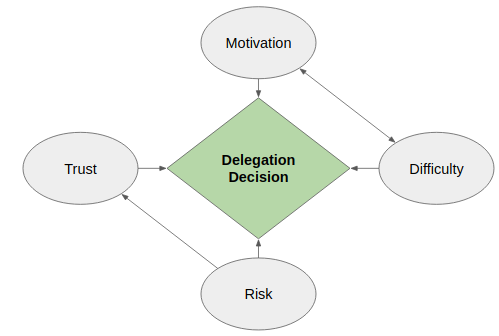
\includegraphics[width=8cm]{model-1.png}
  \label{1}
  \caption{Factors behind task delegability}
\end{figure}

%\subsection{Task Factors}
%\begin{enumerate}
%    \item Task Complexity
%    \item Task Importance (?)
%    \item Task Difficulty
%    \item Task Variability
%\end{enumerate}

\section{Survey Design}
TODO...

For the given task, please evaluate 
\subsection{Purpose}
\subsection{Difficulty}
\subsection{Risk}
\subsection{Trust}


\section{Example}
Example task: "Decide whether or not to release a defendant on bail awaiting trial."

Possible considerations under the framework:
\begin{enumerate}
    \item \textbf{Purpose:} Values may be fairness, justice, and compassion. How do I balance them? Say my goal is to achieve justice while maximizing fairness and compassion. 
    \item \textbf{Difficulty:} I do not have much experience judging since I've never done it. Low self-efficacy, no experience, social skills and law knowledge required, effort to read the files, listen, and decide. 
    \item \textbf{Risk:} As a citizen I'm not accountable individually unless involved with the case. Cost of error is the defendant's freedom and possibly causing their family hardship and heartache, vs. the possible victim if the defendant were to commit (another) crime. The probability of error is high.
    \item \textbf{Trust:} How well do I trust the AI agent to match my values here? 
\end{enumerate}

\section{Survey Data Experiments}

\subsection{Factor Weights and Predictive Model}
Split the 200 tasks into training, validation, and test data (1/3, 1/3, 1/3)? Use the survey results from some of the task data as a training, build a model, and present the accuracy of the model on a held-out test set.

\subsection{Clustering?}
People will use different thought processes and considerations when arriving at a delegation decision. For example, one person may tend to value personal meaning and motivation more than another person, who may favor utility along a more logical cost-benefit analysis. Maybe we can cluster on the factors and labels to produce different types of decision processes. May have to use individual responses rather than averaged task responses for this to work. 

\section{Possible Design Implications}

\subsection{Trust Considerations}
Design decisions meant to improve trust are obviously best-spent on situations in which trust has more weight in delegability decisions. Prior research indicates that such designs may include interpretability, explanations, personality similarity, social norms, but the specific task situations that lend themselves to each of those choices is not in the scope of this paper.

In addition to trust in the AI agent itself, trust may be fostered through intentionality and value-alignment of the system's designer/manufacturer. Accountability on their part helps to align incentives and make value-alignment more likely. Alternatively, institutional trust may be improved in leau of trust in the agent by developing regulations or certifications which people can trust instead [cite].

Finally, if task familiarity and confidence are more likely to lead to reliance, then perhaps explanations of skills or strategies will help to encourage familiarity with both the task and the agent, helping to improve vicarious task knowledge (and thus self-efficacy) as well as trust.

%\section{References}
%The references section should be labeled ``References" and should appear at the very end of the paper (don't end the paper with references, and then put a figure by itself on the last page). A sample list of references is given later on in these instructions. Please use a consistent format for references. Poorly prepared or sloppy references reflect badly on the quality of your paper and your research. Please prepare complete and accurate citations.

\bibliography{cite}
\bibliographystyle{aaai}

\end{document}
